\chapter{Numerical Solution of Adjoint Equations}
\label{chapter-four}

This section details the derivation of the adjoint equations to be solved in
conjunction with the primal flow equations.  The primary goals of this research
are to:
\begin{enumerate}
  \item Compute sensitivities of aerodynamic and aerothermodynamic quantities to
    design variables
  \item Utilize a decoupled approach in the solution of the adjoint
\end{enumerate}
To achieve these goals, the sensitivity to the primal flow equation formulation
must first be solved.  For a discrete adjoint formulation, this requires a
solution of costate variables that relate a change in the flow equation
residuals to a change in the function of interest.  The adjoint solver also
suffers from the quadratic scaling in computational cost and memory required,
similar to the primal flow solver.  To mitigate this scaling, a decoupled scheme
is derived that is consistent with the decoupled flow solver.

\section{Discrete Adjoint Derivation}
\label{sec:adj-derivation}

The derivation for the discrete adjoint begins with forming the Lagrangian as
%------------------------------------------------------------------------------%
\begin{equation}
  L(\md,\mq,\mx,\mathbf{\Lambda})=f(\md,\mq,\mx)
  +\mathbf{\Lambda}^T\mr(\md,\mq,\mx)
  \label{lagrangian}
\end{equation}
%------------------------------------------------------------------------------%
where $\mr$ is the residual of the flow equations, $\md$ is the vector of design
variables, $\mq$ is the vector of conserved variables, and $\mx$ is the mesh
coordinates.  Differentiating with respect to the design variables, $\md$,
yields
%------------------------------------------------------------------------------%
\begin{equation}
  \pd{L}{\md} = 
  \Bigg\{\pd{f}{\md}+\bigg[\pd{\mx}{\md}\bigg]^T \pd{f}{\mx}\Bigg\} 
  + \bigg[\pd{\mq}{\md}\bigg]^T
  \Bigg\{\pd{f}{\mq}+\bigg[\pd{\mr}{\mq}\bigg]^T \mathbf{\Lambda}\Bigg\}
  +\Bigg\{\bigg[\pd{\mr}{\md}\bigg]^T
  +\bigg[\pd{\mx}{\md}\bigg]^T\bigg[\pd{\mr}{\mx}\bigg]^T\Bigg\}\mathbf{\Lambda}
  \label{dL}
\end{equation}
%------------------------------------------------------------------------------%
To eliminate the dependence of conserved variables, $\mq$, on the design
variables, we solve the adjoint equation
%------------------------------------------------------------------------------%
\begin{equation}
  \bigg[\pd{\mr}{\mq}\bigg]^T\mathbf{\Lambda} = -\pd{f}{\mq}
  \label{adjoint-main}
\end{equation}
%------------------------------------------------------------------------------%
Where the Lagrange multipliers (hereafter referred to as costate variables),
$\adjlam{}$, are the cost function dependence on the residual
%------------------------------------------------------------------------------%
\begin{equation}
  \mathbf{\Lambda}=-\pd{f}{\mr}
\end{equation}
%------------------------------------------------------------------------------%
\eref{dL} can ultimately be used in error estimation and sensitivity analysis
for design optimization.  With the second term in \eref{dL} eliminated, the
derivative of the Lagrangian becomes
%------------------------------------------------------------------------------%
\begin{equation}
  \pd{L}{\md}=
  \Bigg\{\pd{f}{\md}+\bigg[\pd{\mx}{\md}\bigg]^T \pd{f}{\mx}\Bigg\}
  +\Bigg\{\bigg[\pd{\mr}{\md}\bigg]^T
  +\bigg[\pd{\mx}{\md}\bigg]^T\bigg[\pd{\mr}{\mx}\bigg]^T\Bigg\}\mathbf{\Lambda}
  \label{obj-function}
\end{equation}
%------------------------------------------------------------------------------%
By solving the adjoint equation (\eref{adjoint-main}) to obtain the costate
variable vector, $\mathbf{\Lambda}$, we can now use a non-linear optimizer to
determine the optimum set of design variables, $\md^*$. This optimization can be
done using {\bf SNOPT\cite{snopt-manual}}, {\bf KSOPT\cite{KSOPT}}, or {\bf
NPSOL\cite{npsol-manual}} in FUN3D, as well as a host of other non-linear
optimizers.

\section{Block Jacobi Adjoint Decoupling}
\label{block-jacobi-decoupling}

It is possible to decouple the adjoint equations in a fashion similar to that
done to the primal flow equations.  In this decoupled adjoint formulation, the
conserved variables are split identically to the flow equations, with the
fully-coupled vector of conserved variables
%------------------------------------------------------------------------------%
\begin{equation}
	\vU =
  \begin{pmatrix}
 		\rho_1    \\
		\vdots    \\
		\rho_{ns} \\
    \rho \vu  \\
		\rho E    \\
	\end{pmatrix}
  \label{all-vars}
 \end{equation}
%------------------------------------------------------------------------------%
 split into
%------------------------------------------------------------------------------%
\begin{equation}
	\begin{matrix}
		\mathbf{U}'=\begin{pmatrix}
			\rho \\
			\rho \vu \\
			\rho E
		\end{pmatrix},\quad &
		\mathbf{\Vhat}=\begin{pmatrix}
			c_1 \\
			\vdots \\
			c_{ns}
		\end{pmatrix}
	\end{matrix}
  \label{dc-vars}
\end{equation}
%------------------------------------------------------------------------------%
With this splitting, the mixture equations for single point in the global system
of the decoupled flow solve can be written as
%------------------------------------------------------------------------------%
\begin{equation}
  \left[ 
  \frac{V}{\Delta t}\mi + 
  \begin{pmatrix}
    \rdiff{\rho}{\rho} & \rdiff{\rho}{\rho \vu} & \rdiff{\rho}{\rho E} \\ \\
    \rdiff{\rho \vu}{\rho} & \rdiff{\rho \vu}{\rho \vu} & \rdiff{\rho \vu}{\rho E} \\ \\
    \rdiff{\rho E}{\rho} & \rdiff{\rho E}{\rho \vu} & \rdiff{\rho E}{\rho E}
  \end{pmatrix}
  \right]
  \begin{pmatrix}
    \Delta \rho \\ \\
    \Delta \rho \vu \\ \\
    \Delta \rho E
  \end{pmatrix}
  =
  \begin{pmatrix}
    \res{\rho} \\ \\
    \res{\rho \vu} \\ \\
    \res{\rho E}
  \end{pmatrix}
  \label{approx-jac}
\end{equation}
%------------------------------------------------------------------------------%
Likewise, the species mass equations for a single point can be written as
%------------------------------------------------------------------------------%
\begin{gather}
  \left[
    \frac{\rho V}{\Delta t}\mi + 
    \begin{pmatrix}
      \rdiff{\rho_1}{c_1} & \cdots & \rdiff{\rho_{1}}{c_{ns}} \\ \\
      \vdots & \ddots & \vdots \\ \\
      \rdiff{\rho_{ns}}{c_1} & \cdots & \rdiff{\rho_{ns}}{c_{ns}}
    \end{pmatrix}
  \right]
  \begin{pmatrix}
    \Delta c_1 \\ \\
    \vdots \\ \\
    \Delta c_{ns}
  \end{pmatrix}
  =
  \begin{pmatrix}
    \resp{\rho_1} \\ \\
    \vdots \\ \\
    \resp{\rho_{ns}}
  \end{pmatrix}
  \label{approx-jac-dc} \\[12pt]
  \resp{\rho_s} = \res{\rho_s} - c_s \res{\rho}
  \label{resp-def} \\[12pt]
  \res{\rho} = \resrho
  \label{resrho-def}
\end{gather}
%------------------------------------------------------------------------------%
\erefs{approx-jac}{approx-jac-dc} omitted dependencies between equation sets,
and it was been found\cite{candler} that omitting these dependencies does not
hinder convergence the primal flow solver.  Because the adjoint requires an
exact linearization of the converged steady-state solution, however, these
cross-system dependencies must be accounted for in the decoupled adjoint
formulation.

The next step is to reconcile the split conserved variables, $\mathbf{U}'$ and
$\Vhat$, with the conserved variable vector $\mq$ in the discrete adjoint
formulation given in \eref{adjoint-main}. This begins by recognizing that the
decoupled scheme can actually also be solved as a fully-coupled system of
equations that involves the change of variables
%------------------------------------------------------------------------------%
\begin{equation}
  \mU = \begin{pmatrix}
    \rho_1 \\
    \vdots \\
    \rho_{ns} \\
    \rho \vu \\
    \rho E
  \end{pmatrix}
  \rightarrow
  \mv = \begin{pmatrix}
    c_1 \\
    \vdots \\
    c_{ns} \\
    \rho \\
    \rho \vu \\
    \rho E
  \end{pmatrix}
  \label{u-v-vars}
\end{equation}
%------------------------------------------------------------------------------%
as well as the change of equations
%------------------------------------------------------------------------------%
\begin{equation}
  \ru{} =
  \begin{pmatrix}
    \res{\rho_1} \\
    \vdots \\
    \res{\rho_{N_s}} \\
    \res{\rho \vu} \\
    \res{\rho E}
  \end{pmatrix}
  \rightarrow
  \rv{} =
  \begin{pmatrix}
    \res{\rho_1} - c_1 \resrho \\
    \vdots \\
    \res{\rho_{N_s}} - c_{N_s} \resrho \\
    \resrho \\
    \res{\rho \vu} \\
    \res{\rho E}
  \end{pmatrix}
  \label{fc-to-dc-res}
\end{equation}
%------------------------------------------------------------------------------%
The derivation of the transformation matrices need to convert between these two
systems are included in \sref{change-of-var-section}.  From this perspective,
the decoupled scheme linear system for the flow solver can be viewed, with no
approximations, as
%------------------------------------------------------------------------------%
\begin{equation}
  \left[ 
    \frac{V}{\Delta t} \mi + 
    \begin{pmatrix}
      \rpdiff{\rho_1}{c_1}      & \dots  & \rpdiff{\rho_1}{c_{N_s}}     & \rpdiff{\rho_1}{\rho}     & \rpdiff{\rho_1}{\rho \vu}     &  \rpdiff{\rho_1}{\rho E}  \\ \\
      \vdots                    & \ddots & \vdots                       & \vdots                    & \vdots                        & \vdots                    \\ \\
      \rpdiff{\rho_{N_s}}{c_1}  & \dots  & \rpdiff{\rho_{N_s}}{c_{N_s}} & \rpdiff{\rho_{N_s}}{\rho} & \rpdiff{\rho_{N_s}}{\rho \vu} &  \rpdiff{\rho_{N_s}}{\rho E}    \\ \\
      \rdiff{\rho}{c_1}         & \dots  & \rdiff{\rho}{c_{N_s}}        & \rdiff{\rho}{\rho}        & \rdiff{\rho}{\rho \vu}        &  \rdiff{\rho}{\rho E}     \\ \\
      \rdiff{\rho \vu}{c_1}     & \dots  & \rdiff{\rho \vu}{c_{N_s}}    & \rdiff{\rho \vu}{\rho}    & \rdiff{\rho \vu}{\rho \vu}    &  \rdiff{\rho \vu}{\rho E} \\ \\
      \rdiff{\rho E}{c_1}       & \dots  & \rdiff{\rho E}{c_{N_s}}      & \rdiff{\rho E}{\rho}      & \rdiff{\rho E}{\rho \vu}      &  \rdiff{\rho E}{\rho E}
    \end{pmatrix}
  \right]
  \begin{pmatrix}
    \Delta c_1      \\ \\
    \vdots     \\ \\
    \Delta c_{N_s}  \\ \\
    \Delta \rho     \\ \\
    \Delta \rho \vu \\ \\
    \Delta \rho E
  \end{pmatrix}
  =
  \begin{pmatrix}
    \res{\rho_1}^{'}     \\ \\
    \vdots               \\ \\
    \res{\rho_{N_s}}^{'} \\ \\
    \res{\rho}           \\ \\
    \res{\rho \vu}       \\ \\
    \res{\rho E}
  \end{pmatrix}
  \label{dc-full-system}
\end{equation}
%------------------------------------------------------------------------------%
In addition to \erefs{dfdvl}{dfdvr}, the iterative mechanism used in the flow
solver makes the following approximations to the Jacobians
%------------------------------------------------------------------------------%
\begin{equation}
  \begin{aligned}
    \rdiff{\rho}{c_s} &= \rdiff{\rho \vu}{c_s} = \rdiff{\rho E}{c_s} &= 0 \\[6pt]
    \rpdiff{\rho_s}{\rho} &= \rpdiff{\rho_s}{\rho \vu} = \rpdiff{\rho_s}{\rho E} &= 0
  \end{aligned}
  \label{dc-approximations}
\end{equation}
%------------------------------------------------------------------------------%
which results in a significantly sparser matrix
%------------------------------------------------------------------------------%
\begin{equation}
  \left[ 
    \frac{V}{\Delta t} \mi + 
    \left(
    \begin{array}{c c c | c c c }
      \rdiff{\rho_1}{c_1}      & \dots  & \rdiff{\rho_1}{c_{N_s}} & & & \\[12pt]
      \vdots                    & \ddots & \vdots                       & & 0 & \\[12pt]
      \rdiff{\rho_{N_s}}{c_1}  & \dots  & \rdiff{\rho_{N_s}}{c_{N_s}} & & & \\[12pt]
      \hline
      & & & & & \\
      & & & \rdiff{\rho}{\rho}        & \rdiff{\rho}{\rho \vu}        &  \rdiff{\rho}{\rho E}     \\[12pt]
      & 0 & & \rdiff{\rho \vu}{\rho}    & \rdiff{\rho \vu}{\rho \vu}    &  \rdiff{\rho \vu}{\rho E} \\[12pt]
      & & & \rdiff{\rho E}{\rho}      & \rdiff{\rho E}{\rho \vu}      &  \rdiff{\rho E}{\rho E}
    \end{array}
    \right)
  \right]
  \begin{pmatrix}
    \Delta c_1      \\ \\
    \vdots     \\ \\
    \Delta c_{N_s}  \\ \\
    \Delta \rho     \\ \\
    \Delta \rho \vu \\ \\
    \Delta \rho E
  \end{pmatrix}
  =
  \begin{pmatrix}
    \res{\rho_1}^{'}     \\ \\
    \vdots               \\ \\
    \res{\rho_{N_s}}^{'} \\ \\
    \res{\rho}           \\ \\
    \res{\rho \vu}       \\ \\
    \res{\rho E}
  \end{pmatrix}
  \label{dc-sparse-system}
\end{equation}
%------------------------------------------------------------------------------%
that results in the approximate factorization used by the flow solver.  This is
a more complete picture of the decoupled scheme, but it indicates that
\eref{dc-full-system} must be used to formulate the adjoint system of equations,
since \eref{dc-sparse-system} omits a significant part of the Jacobian.

The simplest approach to solving \eref{adjoint-main} with system of equations
$\rv{}$ and dependent variables $\mv$ is to solve
%------------------------------------------------------------------------------%
\begin{equation}
  \pd{\rv{}}{\mv}^{\mathsmaller T}\adjlam{\mv} = -\pd{f}{\mv}
  \label{v-adj}
\end{equation}
%------------------------------------------------------------------------------%
directly, via a linear solver such as GMRES \cite{saad1986gmres}.  Nielsen
\cite{nielsenPhD} found that time-marching the FUN3D discrete adjoint linear
system with the same point-implicit scheme as the FUN3D flow solver was more
robust, and solved systems where GMRES tended to stall.  The time marching
algorithm also has the benefit of reusing the approximate Jacobians from the
flow solver, transforming \eref{v-adj} into
%------------------------------------------------------------------------------%
\begin{equation}
  \left(
    \frac{V}{\Delta t} \mi + \drvdv
  \right)^{\mathsmaller T}
  \Delta \adjlam{\mv}
  =
  -\left(\pd{\rv{}}{\mv}^{\mathsmaller T}\adjlam{\mv} + \pd{f}{\mv} \right)
  \label{v-adj-time}
\end{equation}
%------------------------------------------------------------------------------%
where $\drvdv$ can include all of the Jacobian approximations used by the flow
solver Jacobians, including those in \eref{dc-approximations}.
\eref{v-adj-time} can be solved using the same iterative mechanism
as the flow solver; however, the exact linearizations of $\pd{\rv{}}{\mv}$
are different and more complex than the linearizations required by the
traditional fully-coupled system, $\pd{\ru{}}{\mU}$.  This makes the decoupled
scheme somewhat less attractive, since the re-implementing the exact
linearizations for the change of variable and change of equations in the
decoupled scheme requires a significant amount of coding and verification.  An
alternative to \eref{v-adj-time} is to recast the decoupled scheme again as a
series of matrix transformations on the fully-coupled system of equations.  For
the flow solver this involves
%------------------------------------------------------------------------------%
\begin{equation}
  \begin{aligned}
    \left( \frac{V}{\Delta t} \mi + \pd{\ru{}}{\mU} \right) \Delta \mU &= \ru{} \\[12pt]
    \pd{\rv{}}{\ru{}}
    \left( \frac{V}{\Delta t} \mi + \pd{\ru{}}{\mU} \right)
    \left( \pd{\mU}{\mv} \right) \Delta \mv
    &= 
    \pd{\rv{}}{\ru{}} \ru{}
  \end{aligned}
  \label{fc-to-dc-flow}
\end{equation}
%------------------------------------------------------------------------------%
From the perspective of \eref{fc-to-dc-flow}, the decoupled flow solver scheme
is actually the result of left and right preconditioning on the fully-coupled
scheme that can be generically written as
%------------------------------------------------------------------------------%
\begin{equation}
  \begin{aligned}
    \mm \left(\frac{V}{\Delta t} \mi + \ma_{\mU} \right) 
    \left( \mb \Delta \mv \right) &= \mm \ru{} \\
    \Delta \mU &= \mb \Delta \mv
  \end{aligned}
  \label{generic-fc-to-dc}
\end{equation}
%------------------------------------------------------------------------------%
where $\mm$ is the left preconditioner, $\pd{\rv{}}{\ru{}}$, $\mb$ is the right
preconditioner, $\pd{\mU}{\mv}$, and $\ma_{\mU}$ is the Jacobian matrix for the
fully coupled system, $\pd{\ru{}}{\mU}$.  A full derivation of the
transformation of variables sets, $\pd{\mU}{\mv}$ is included in
\aref{change-of-var-section}. \eref{generic-fc-to-dc} is crucial towards the
understanding of the adjoint system of equations, since the transpose operation
will reverse the order of operations of these matrix products.  Based on
\eref{generic-fc-to-dc}, the Jacobian for the system based on $\rv{}$ and $\mv$,
denoted as $\ma_{\mv}$, can be written as
%------------------------------------------------------------------------------%
\begin{equation}
  \ma_{\mv} = \mm \ma_{\mU} \mb
  \label{adj-dc-generic}
\end{equation}
%------------------------------------------------------------------------------%
along with its transpose
%------------------------------------------------------------------------------%
\begin{equation}
  \ma_{\mv}^{T}
   = \left( \mm \ma_{\mU} \mb \right)^{T}
   = \mb^{T} \ma_{\mU}^{T} \mm^{T}
  \label{adj-dc-generic-transpose}
\end{equation}
%------------------------------------------------------------------------------%
Thus, in the adjoint linear system of equations, $\mb$ becomes the left
preconditioner, and $\mm$ becomes the right preconditioner.  Applying the matrix
operations in \eref{adj-dc-generic-transpose}, \eref{v-adj} can be re-written as
%------------------------------------------------------------------------------%
\begin{equation}
  \left( \pd{\mU}{\mv} \right)^{T}
  \left(\pd{\ru{}}{\mU} \right)^{T} 
  \left( \pd{\rv{}}{\ru{}} \right)^{T}
  \adjlam{\mv} 
  = 
  - \left( \pd{\mU}{\mv} \right)^{T}
  \left( \pd{f}{\mU} \right)
  \label{adj-u-to-v}
\end{equation}
%------------------------------------------------------------------------------%
and applying the same time-marching strategy as \eref{v-adj-time} leads to
%------------------------------------------------------------------------------%
\begin{equation}
  \left(
    \frac{V}{\Delta t} \mi + \drvdv
  \right) \Delta \adjlam{\mv}
  = -
  \left( \pd{\mU}{\mv} \right)^{T}
  \left[
    \left(\pd{\ru{}}{\mU} \right)^{T} 
    \left( \pd{\rv{}}{\ru{}} \right)^{T}
    \adjlam{\mv} 
    + \left( \pd{f}{\mU} \right)
  \right]
  \label{adj-u-to-v-time}
\end{equation}
%------------------------------------------------------------------------------%
Where the adjoint costate variables associated with the fully coupled equations,
$\ru{}$ can be recovered from the right preconditioning
%------------------------------------------------------------------------------%
\begin{equation}
  \Delta \adjlam{\mU} = \pd{\ru{}}{\rv{}} \Delta \adjlam{\mv}
  \label{adj-lam-v-to-u}
\end{equation}
%------------------------------------------------------------------------------%
Based on \erefs{adj-u-to-v-time}{adj-lam-v-to-u}, it is possible to reuse the
exact Jacobian of the fully coupled scheme, $\ma_{\mU}$, instead of computing
the exact Jacobian of the decoupled system, $\ma_{\mv}$.  This reused is very
attractive, since the implementation of the fully coupled scheme does not need
to be changed at the low-level linearizations.  Instead, the residual of the
adjoint can be formed in the exact same fashion as the fully coupled scheme, and
a series of matrix operations can then be performed to transform the equations
and dependent variables into those used by the decoupled scheme. A full
derivation of the change of equation sets, $\pd{\ru{}}{\rv{}}$, is included
in \aref{sec:change-of-equations}

The iterative mechanism required by the adjoint solver has been found to be much
more flexible than the flow solver.  In the flow solver, the mixture variables
were updated before the species mass fractions, with the former used to compute
the later at the next time level.  This same process can be carried out on the
costate variable vector, $\adjlam{\mv}$, in the adjoint solver, which would
correspond to a block Gauss-Seidel type scheme; however, through testing, their
is no significant advantage found applying costate variables at the next time
level to compute costate variables at the previous time level.  Thus, the much
more cost effective approach is to apply a block jacobi scheme where all
costate variables are updated at the same time level, regardless of order.
Because information is not passed between the costate variables for the mixture
equations and costate variables for the species equations, only a single
residual vector is required to be computed per timestep in the block jacobi
adjoint solver, rather than two required by a block gauss-seidel type adjoint
solver.  This algorithm is also more efficient than the flow solver iterative
mechanism, which requires two residual vectors to be computed per timestep.


\section{Higher-order Reconstruction Linearizations}
\label{sec:higher-order-linearizations}

The reconstruction scheme detailed in \sref{sec:2nd-order-reconstruction} must
be exactly linearized in the adjoint solver to achieve correct sensitivity
derivatives. The adjoint uses a frozen flux limiter, for purposes that will be
discussed in a later section, and is therefore held as constant in the
linearization computations.  All gradient information in \eref{u-muscl},
$\pd{q_{1,2}}{x}$, $\pd{q_{1,2}}{y}$, and $\pd{q_{1,2}}{z}$, are computed using
least-squares.  For the example stencil shown in \fref{fig:lsq-gradients} this
is effectively computed as
%------------------------------------------------------------------------------%
\begin{equation}
  \begin{aligned}
    \pd{q}{x} &= \sum_{i=1}^{5}{W_{x,i}\left( q_i - q_0 \right)} \\
    \pd{q}{y} &= \sum_{i=1}^{5}{W_{y,i}\left( q_i - q_0 \right)} \\
    \pd{q}{z} &= \sum_{i=1}^{5}{W_{z,i}\left( q_i - q_0 \right)}
  \end{aligned}
  \label{grad-construction}
\end{equation}
%------------------------------------------------------------------------------%
where the $z$ direction would come from geometry out of the page.
%------------------------------------------------------------------------------%
\begin{figure}[h]
  \centering
  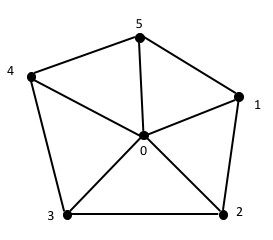
\includegraphics[width=0.5\textwidth]{figures/stencil.png}
  \caption{Example Stencil for Least-Squares Gradient Evaluation}
  \label{fig:lsq-gradients}
\end{figure}
%------------------------------------------------------------------------------%
In practice, the higher order linearizations can be managed easily by
constructing a list of neighboring nodes for each node.  By the chain rule the
linearization of the residual, $\mr$, is then evaluated in two parts
%------------------------------------------------------------------------------%
\begin{equation}
  \pd{\vR\left(\mq^*\left( \mq \right) \right)}{\mq} = 
  \pd{\vR}{\mq} + \pd{\vR}{\mq^{*}}\pd{\mq^*}{\mq}
  \label{residual-high-low}
\end{equation}
%------------------------------------------------------------------------------%
where $\mq$ are the conserved variables at each node, and $\mq^*$ are the higher
order terms computed in the U-MUSCL reconstruction; therefore, after computing
the exact first-order Jacobian of the Roe FDS scheme, $\pd{\vR}{\mq}$, the
higher order linearizations are computed by making a circuit around each node to
pick up the contributions from the least squares gradient computation.  For the
example stencil in \fref{fig:lsq-gradients}, the contribution to the residual
from looping around node 0 would be
%------------------------------------------------------------------------------%
\begin{equation}
  \pd{\vR_0}{\mq^*}\pd{\mq^*}{\mq_0} = \pd{\vR_0}{\mq^*} \left[\sum_{i=1}^5{(1-\kappa)
  \left( -W_{x,i}dx - W_{y,i}dy - W_{z,i}dz \right) \pd{q_0}{\mq_0}}\right]
  \label{ho-linearization}
\end{equation}
%------------------------------------------------------------------------------%
An important point that this illustrates is that the form of the higher order
linearizations does not change significantly based on the primitive variable
vector $q$, only affecting the primitive to conserved variable Jacobian,
$\pd{q_0}{\mq_0}$, which is easily computed.  This is a powerful telescoping
property of the reconstruction scheme from \sref{sec:2nd-order-reconstruction},
and it significantly decreases the complexity of the code required to implement
the second order term linearizations.  The downside of looping around each node
is the high number of cache misses, as the data structures in FUN3D are not
conducive to co-locating memory based on stencil.  This results in the
evaluation of the second order linearizations being the dominant computational
cost in the adjoint solver.

\section{Memory and Computational Cost of Exact Second Order Linearizations}
\label{sec:2nd-order-mem-cost}

As shown in \sref{sec:higher-order-linearizations}, the second order
reconstruction results in an extended stencil.  This significantly decreases the
sparsity of the Jacobian, since the linearizations at node must now include the
nearest neighbors.  The cost of computing these linearizations can quickly
dominate other costs of the adjoint, but can be significantly mitigated if the
linearizations of second order Jacobian are stored.  This essentially trades all
the memory in the simulation for computational speed, and may not be possible
for large mesh sizes.  Since all of the linearizations in the second order
Jacobian must be exact, the memory saving approximations of the decoupled scheme
can only be applied to the LHS Jacobians in \eref{adj-u-to-v-time}.  This last
point makes the quadratic scaling of memory required with the number of species
a significant concern of the adjoint.  The savings provided by the decoupled
scheme become a very significant benefit in cases involving many species, since
the memory freed by the sparsity on the LHS of \eref{adj-u-to-v-time} can be
used by the RHS linearizations to increase in computational efficiency.
